\documentclass[../main.tex]{subfiles}
\begin{document}
\chapter{Analisi del problema}

\section{Network flows}


Le misurazioni del traffico sono necessarie per gestire tutti i tipi di reti IP. L'amministratore delle reti ha bisogno di una vista dettagliata del traffico di rete per ragioni di sicurezza, contabilità e gestione. Le composizioni del traffico devono essere analizzate accuratamente quando si valutano le metriche del traffico o quando si riscontrano problemi di rete.

Tutte queste misurazioni devono essere fatte analizzando tutti i pacchetti che scorrono verso i punti centrali della rete come router o switch. L'analisi di questi pacchetti può essere eseguita all'istante o registrando tutti i pacchetti e analizzarli in un secondo momento. Con l'aumento delle capacità di rete e dei volumi di traffico questo tipo di approccio non è molto efficiente. 

Invece i pacchetti simili (pacchetti con un insieme di proprietà comuni) possono essere raggruppati insieme per la composizioni di \textit{flows}. Un \textit{flow} può essere composto da tutti i pacchetti che condividono la stessa origine e l'indirizzo di destinazione, in questo modo tipi simili di traffico possono essere memorizzati in un formato più compatto senza perdere le informazioni a cui siamo interessati.

Una volta raccolte queste informazioni si ha una vista dettagliata del traffico di rete. 

\subsection{Architettura Network Flow}
Il core del modello di misurazione del traffico sono entità di rete chiamate \textit{metri} del traffico. I contatori osservano i pacchetti mentre passano per un singolo punto sulla loro rete e li classificano in determinati gruppi. Per chiascun gruppo di questo tipo, un misuratore accumula deterinati attributi, ad esempio il numero di pacchetti e byte osservati per il gruppo. Questi gruppi di traffico possono corrispondere a un utente, un sistema host, una rete, un gruppo direti, un particolare indirizzo di trasporto, qualsiasi combinazione di quanto sopra. \newline

Ai fini della misurazione del flusso del traffico, definiamo il concetto di \textit{network flow}, che è come un equivalente logico artificiale di una chiamata o di una connessione. Un flusso è una porzione di traffico, delimitata da un orario di inizio e di fine, che appartiene a uno dei gruppi di traffico a consumo sopra menzionati. \newline [http://www.ietf.org/rfc/rfc2722.txt]

Per i protocolli di rete senza connessione come IP non esiste per definizione alcun modo per stabilire se un pacchetto con una particolare combinazione sorgente - destinazione fa parte di un flusso di pacchetti o non, ogni pacchetto è completamente indipendente. Un contatore di traffio ha, come parte della sua configurazione, un insieme di regole che specificano i flussi di interesse, in termine dei valori dei loro attributi. Deriva i valori degli attributi da ciascun pacchetto osservato e li utilizza per decidere a quale flusso appartengono. Classificare i pacchetti in \textit{flows} in questo modo fornisce un modo economico e pratico per misurare il traffico di rete e suddividerlo in gruppi ben definiti.

\paragraph{Attributi dei Flows}
Ogni contatore del traffico mantiene una tabella con i record dei \textit{flows}. Un record contiene i valori degli attributi di interesse per il suo \textit{flow}. Questi attributi potrebbero includere
\begin{itemize}
				\item \textbf{Indirizzi} per la sorgente e la destinazione dei \textit{flows}. Questi comprendono il tipo di protocollo, gli indirizzi di sorgente e destinazione a vari livelli della rete (estratti dall'intestazione del pacchetto) e il numero dell'interfaccia su cui è stato osservato il pacchetto.
				\item \textbf{Orario} su cui sono stati visualizzati i pacchetti per questo flusso, vale a dire i tempi di creazione e ultima attività del flusso.
				\item \textbf{Direzione} del traffico dei \textit{flows} 
\end{itemize}


Il gruppo di traffico di un flusso è specificato dai valori dei suoi attributi \textbf{Indirizzo}. Ad esempio, se gli attributi di un indirizzo di flusso sono stati specificati come "indirizzo sorgente = indirizzo IP 10.1.0.1, indirizzo di destinazione = indirizzo IP 26.1.0.1", in tale flusso verranno conteggiati solo i pacchetti IP da 10.1.0.1 a 26.1.0.1 e viceversa.


\section{Argus}

\textit{Audit Record Generation and Utilization System} è la prima implementazione del monitoraggio dei flussi di rete ed è un progetto di monitoraggio continuo del flusso di rete open source. \newline

Questo programma è utilizzato da \textit{Stratosphere IPS} e di conseguenza accetta in input file che rispettano il formato di \textit{Argus}. Questi file hanno estensione \textit{*.binetflow} e hanno un header formato da 17 campi, separati dal carattere ","
\begin{table}[H]
\begin{tabular}{|l|l|}
\hline
\textbf{campo} & \textbf{descrizione}                    \\ \hline
StartTime      & record start time                       \\ \hline
Dur            & record total duration                   \\ \hline
Proto          & transaction protocol                    \\ \hline
SrcAddr        & source IP address                       \\ \hline
Sport          & source port number                      \\ \hline
Dir            & direction of transaction                \\ \hline
DstAddr        & destination IP address                  \\ \hline
Dport          & destination port number                 \\ \hline
State          & transaction state                       \\ \hline
sTos           & source TOS byte value                   \\ \hline
dTos           & destination TOS byte value              \\ \hline
TotPkts        & total transaction packet count          \\ \hline
TotBytes       & total transaction bytes                 \\ \hline
SrcBytes       & src -\textgreater dst transaction bytes \\ \hline
srcUdata       & source user data buffer                 \\ \hline
dstUdata       & destination user data buffer            \\ \hline
Label          & metadata label                          \\ \hline
\end{tabular}
\end{table}

\section{nProbe}

Negli ambienti commerciali, \textit{NetFlow} è probabilmente lo standard \textit{de facto} per la contabilità e la fatturazione del traffico di rete. \textit{NetFlow} è una tecnologia creata originariamente da Cisco e ora è standardizzata come \textit{Internet Protocol Flow Information eXport} \newline
Il \textit{DIEF} utilizza \textit{nProbe} per la cattura e l'analisi dei pacchetti di reti. La cattura dei pacchetti viene salvata su file che hanno formato proprietario, con estensione \textit{*.flows}.
Questo formato ha un header formato da 29 campi, ciascun campo è separato da un carattere speciale.

\begin{table}[H]
\begin{tabular}{|l|l|}
\hline
\multicolumn{1}{|c|}{\textbf{campo}} & \multicolumn{1}{c|}{\textbf{descrizione}}     \\ \hline
IPV4\_SRC\_ADDR                      & IPv4 source address                           \\ \hline
IPV4\_DST\_ADDR                      & IPv4 destination address                      \\ \hline
IPV4\_NEXT\_HOP                      & IPv4 next hop address                         \\ \hline
INPUT\_SNMP                          & input interface SNMP idx                      \\ \hline
OUTPUT\_SNMP                         & output interface SNMP idx                     \\ \hline
IN\_PKTS                             & incoming flow packets (src -\textgreater dst) \\ \hline
IN\_BYTES                            & incoming flow bytes (src -\textgreater dst)   \\ \hline
FIRST\_SWITCHED                      & SysUptime (msec) of the first flow pkt        \\ \hline
LAST\_SWITCHED                       & SysUptime (msec) of the last flow pkt         \\ \hline
L4\_SRC\_PORT                        & IPv4 source port                              \\ \hline
L4\_DST\_PORT                        & IPv4 destination port                         \\ \hline
TCP\_FLAGS                           & cumulative of all flow TCP flags              \\ \hline
PROTOCOL                             & IP protocol byte                              \\ \hline
SRC\_TOS                             & Type of service byte                          \\ \hline
SRC\_AS                              & source BGP AS                                 \\ \hline
DST\_AS                              & destination BGP AS                            \\ \hline
IPV4\_SRC\_MASK                      & IPv4 source subnet mask                       \\ \hline
IPV4\_DST\_MASK                      & IPv4 dest subnet mask                         \\ \hline
L7\_PROTO                            & layer 7 protocol (numeric)                    \\ \hline
BIFLOW\_DIRECTION                    & 1=initiator, 2=reverseInitiator               \\ \hline
FLOW\_START\_SEC                     & seconds (epoch) of the first flow packet      \\ \hline
FLOW\_END\_SEC                       & seconds (epoch) of the last flow packet       \\ \hline
OUT\_PKTS                            & outgoing flow packets (dst -\textgreater src) \\ \hline
OUT\_BYTES                           & outgoing flow bytes (dst -\textgreater src)   \\ \hline
FLOW\_ID                             & serial flow identifier                        \\ \hline
FLOW\_ACTIVE\_TIMEOUT                & activity timeout of flow cache entries        \\ \hline
FLOW\_INACTIVE\_TIMEOUT              & inactivity timeout of flow cache entries      \\ \hline
IN\_SRC\_MAC                         & source MAC address                            \\ \hline
OUT\_DST\_MAC                        & destination MAC address                       \\ \hline
\end{tabular}
\end{table}

\section{Stratosphere IPS}
In questa tesi si è utilizzato Stratosphere Testing Framework, un \textit{Network Intrusion Detection System} che genera modelli comportamentali delle connessioni di reti. Il suo obiettivo è aiutare i ricercatori a trovare nuovi comportamenti malware, etichettare tali comportamenti, creare i loro modelli di traffico e verificare gli algoritmi di rilevamento. Stf funziona utilizzando algoritmi di apprendimento automatico sui modelli comportamentali.

L'obiettivo di Stratosphere Project è quello di creare un \textit{IDS} comportamentale in grado di rilevare e bloccare i comportamenti dannosi nella rete.

Come parte di questo progetto, stf viene utilizzato per generare modelli altamente attendibili di traffico dannoso consentendo una verifica automatica delle prestazioni di rilevamento. \newline

\textit{Stratosphere IPS} non è strettamente un \textit{IPS} nel senso che può impedire l'intrusione. Usa l'acronimo \textit{IPS} perchè l'\textit{IPS} di Stratosphere può bloccare connessioni malevoli usando il firewall del computer. Tuttavia, a causa della natura delle connessioni di traffico, l'\textit{IPS} di Stratosphere necessita di un po' di tempo per rilevare il comportamento dannoso e quindi non può bloccare i primi pacchetti nella connessione.

L'\textit{IPS} di Stratosphere è in grado di rilevare e bloccare connessioni di rete molto fini e pericolose, e quindi dovrebbe essere visto come un complemento delle attuali misure di sicurezza della rete.

\subsection{Il significato dei modelli comportamentali} 
Il nucleo di \textit{Stratosphere IPS} è composto dai modelli comportamentali di reti e algoritmi di rilevamento. I modelli comportamentali rappresentano ciò che una connessione specifica fa nella rete durante la sua vita. Il comportamento è costuito analizzando la sua periodicità, le dimensioni e la durata di ciascun flusso. Sulla base di queste caratteristiche a ciascun flusso viene assegnata una lettera e il gruppo di lettere caratterizza il comportamento della connessione.

Prendiamo come esempio una connessione generata da una botnet che ha il seguente modello comportamentale
\begin{lstlisting}[language=bash]
88*y*y*i*H*H*H*y*0yy*H*H*H*y*y*y*y*H*h*y*h*h*H*H*h*H*y*y*y*H*
\end{lstlisting}

Questa catena di stati che chiamiamo modello comportamentale evidenzia alcune delle caratteristiche del canale C\&C. In questo caso ci dice che i flussi sono altamente periodici (lettere \textit{h}, \textit{i}), con qualche periodicità persa vicino all'inizio (lettere \textit{y}). I flussi hanno anche una grande dimensione con una durata media. I simboli tra le lettere sono correlati al tempo trascorso tra i flussi. In questo caso il simbolo '\textit{*}' significa che il flusso è separato da meno di un'ora. Guardando le lettere si può vedere che questa è una connessione piuttosto periodica, e controllando efficacemente i suoi flussi confermiamo tale ipotesi.
Con l'utilizzo di questo tipo di modelli siamo in grado di generare le caratteristiche comportamentali di un gran numero di azioni dannose. L'immagine seguente mostra i criteri di assegnazione delle lettere per i modelli comportamentali \newline
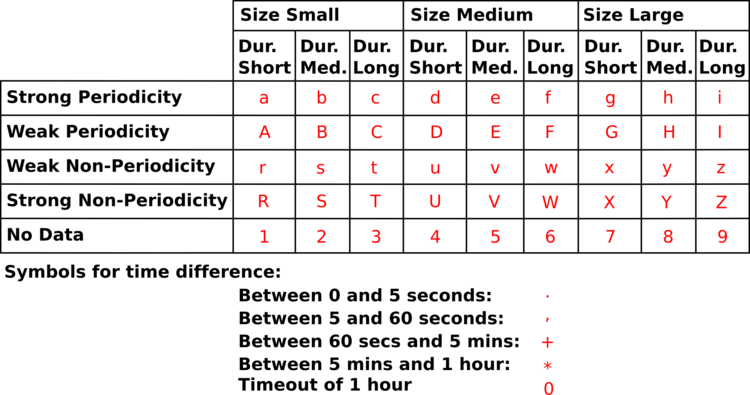
\includegraphics[scale=0.5]{modello-comportamentale.png}


Gli algoritmi di rilevamento utilizzano modelli comportamentali proprietari dannosi per rilevare nuove connessioni sospette nella rete. Il rilevamento viene attualmente eseguito utilizzando algoritmi basati su catene di \textit{Markov}.
La prima parte dell'algoritmo consiste nell'apprendimento e nell'etichettatura del traffico di verità di base. Questo traffico viene utilizzato per creare modelli verificati di comportamenti di rete noti e stabili. \newline

La seconda parte dell'algoritmo consiste nell'utilizzare questi modelli di verità di base noti e verificati per rilevare comportamenti simili in reti sconosciute. \textit{Stratosphere IPS} catturerà il traffico in un computer client e confronterà ogni connessione sconosciuta con i modelli conosciuti di comportamento del traffico. Poichè il modo in cui viene effettuato il rilevamento e come vengono creati i modelli, ciascun modello comportamentale può corrispondere a un'ampia gamma di comportamenti simili senza essere troppo generico. I modelli sono quindi utili per trovare comportamenti simili senza il rischio di generare troppi falsi positivi.


\section{Problematiche dovute all'utilizzo di due diversi formati}
Come si è potuto notare nelle sezioni \textit{2.2} e \textit{2.3}, gli header di \textit{nProbe} ed \textit{Argus} presentano delle differenze che non permettono di essere utilizzati in modo intercambiabile. I file che produce in output \textit{Argus} presentano 17 cambi, ben 12 in meno rispetto ai file di output prodotti da \textit{nProbe}.
L'utilizzazione di due diversi formati presenta errori quando si cerca di utilizzare file prodotti da \textit{nProbe} in Stratosphere IPS. \newline

Questa incompatibilità ha portato alla necessità di una conversione: i file prodotti dal \textit{DIEF} devono essere convertiti in file di formato usato da \textit{Argus}. Questa conversione deve essere efficiente e precisa.

\section{Presentazione del problema}
Il \textit{DIEF} salva i file in una struttura gerarchica fissa ben definita: ci sono 4 livelli di subdir, in cui il primo livello indica l'anno, il secondo il mese, il terzo il giorno e il quarto l'ora. All'interno dell'ultima subdir, quella delle ore, ci sono 60 file uno per ogni minuto della giornata.

\begin{forest}
  for tree={
    font=\ttfamily,
    grow'=0,
    child anchor=west,
    parent anchor=south,
    anchor=west,
    calign=first,
    inner xsep=7pt,
    edge path={
      \noexpand\path [draw, \forestoption{edge}]
      (!u.south west) +(7.5pt,0) |- (.child anchor) pic {folder} \forestoption{edge label};
    },
    before typesetting nodes={
      if n=1
        {insert before={[,phantom]}}
        {}
    },
    fit=band,
    before computing xy={l=15pt},
  }  
[folder structure
  [years
    [months
        [days
            [hours]
        ]
    ]
  ]
]
\end{forest} \newline \newline

I file dei minuti sono compressi usando il programma \textit{gzip}, pertanto c'è da tenerne conto nella soluzione per la conversione.
\end{document}
